\documentclass[]{article}
\usepackage{lmodern}
\usepackage{amssymb,amsmath}
\usepackage{ifxetex,ifluatex}
\usepackage{fixltx2e} % provides \textsubscript
\ifnum 0\ifxetex 1\fi\ifluatex 1\fi=0 % if pdftex
  \usepackage[T1]{fontenc}
  \usepackage[utf8]{inputenc}
\else % if luatex or xelatex
  \ifxetex
    \usepackage{mathspec}
  \else
    \usepackage{fontspec}
  \fi
  \defaultfontfeatures{Ligatures=TeX,Scale=MatchLowercase}
\fi
% use upquote if available, for straight quotes in verbatim environments
\IfFileExists{upquote.sty}{\usepackage{upquote}}{}
% use microtype if available
\IfFileExists{microtype.sty}{%
\usepackage{microtype}
\UseMicrotypeSet[protrusion]{basicmath} % disable protrusion for tt fonts
}{}
\usepackage[margin=1in]{geometry}
\usepackage{hyperref}
\hypersetup{unicode=true,
            pdftitle={Homework 9},
            pdfauthor={Christophe Hunt},
            pdfborder={0 0 0},
            breaklinks=true}
\urlstyle{same}  % don't use monospace font for urls
\usepackage{color}
\usepackage{fancyvrb}
\newcommand{\VerbBar}{|}
\newcommand{\VERB}{\Verb[commandchars=\\\{\}]}
\DefineVerbatimEnvironment{Highlighting}{Verbatim}{commandchars=\\\{\}}
% Add ',fontsize=\small' for more characters per line
\usepackage{framed}
\definecolor{shadecolor}{RGB}{248,248,248}
\newenvironment{Shaded}{\begin{snugshade}}{\end{snugshade}}
\newcommand{\KeywordTok}[1]{\textcolor[rgb]{0.13,0.29,0.53}{\textbf{{#1}}}}
\newcommand{\DataTypeTok}[1]{\textcolor[rgb]{0.13,0.29,0.53}{{#1}}}
\newcommand{\DecValTok}[1]{\textcolor[rgb]{0.00,0.00,0.81}{{#1}}}
\newcommand{\BaseNTok}[1]{\textcolor[rgb]{0.00,0.00,0.81}{{#1}}}
\newcommand{\FloatTok}[1]{\textcolor[rgb]{0.00,0.00,0.81}{{#1}}}
\newcommand{\ConstantTok}[1]{\textcolor[rgb]{0.00,0.00,0.00}{{#1}}}
\newcommand{\CharTok}[1]{\textcolor[rgb]{0.31,0.60,0.02}{{#1}}}
\newcommand{\SpecialCharTok}[1]{\textcolor[rgb]{0.00,0.00,0.00}{{#1}}}
\newcommand{\StringTok}[1]{\textcolor[rgb]{0.31,0.60,0.02}{{#1}}}
\newcommand{\VerbatimStringTok}[1]{\textcolor[rgb]{0.31,0.60,0.02}{{#1}}}
\newcommand{\SpecialStringTok}[1]{\textcolor[rgb]{0.31,0.60,0.02}{{#1}}}
\newcommand{\ImportTok}[1]{{#1}}
\newcommand{\CommentTok}[1]{\textcolor[rgb]{0.56,0.35,0.01}{\textit{{#1}}}}
\newcommand{\DocumentationTok}[1]{\textcolor[rgb]{0.56,0.35,0.01}{\textbf{\textit{{#1}}}}}
\newcommand{\AnnotationTok}[1]{\textcolor[rgb]{0.56,0.35,0.01}{\textbf{\textit{{#1}}}}}
\newcommand{\CommentVarTok}[1]{\textcolor[rgb]{0.56,0.35,0.01}{\textbf{\textit{{#1}}}}}
\newcommand{\OtherTok}[1]{\textcolor[rgb]{0.56,0.35,0.01}{{#1}}}
\newcommand{\FunctionTok}[1]{\textcolor[rgb]{0.00,0.00,0.00}{{#1}}}
\newcommand{\VariableTok}[1]{\textcolor[rgb]{0.00,0.00,0.00}{{#1}}}
\newcommand{\ControlFlowTok}[1]{\textcolor[rgb]{0.13,0.29,0.53}{\textbf{{#1}}}}
\newcommand{\OperatorTok}[1]{\textcolor[rgb]{0.81,0.36,0.00}{\textbf{{#1}}}}
\newcommand{\BuiltInTok}[1]{{#1}}
\newcommand{\ExtensionTok}[1]{{#1}}
\newcommand{\PreprocessorTok}[1]{\textcolor[rgb]{0.56,0.35,0.01}{\textit{{#1}}}}
\newcommand{\AttributeTok}[1]{\textcolor[rgb]{0.77,0.63,0.00}{{#1}}}
\newcommand{\RegionMarkerTok}[1]{{#1}}
\newcommand{\InformationTok}[1]{\textcolor[rgb]{0.56,0.35,0.01}{\textbf{\textit{{#1}}}}}
\newcommand{\WarningTok}[1]{\textcolor[rgb]{0.56,0.35,0.01}{\textbf{\textit{{#1}}}}}
\newcommand{\AlertTok}[1]{\textcolor[rgb]{0.94,0.16,0.16}{{#1}}}
\newcommand{\ErrorTok}[1]{\textcolor[rgb]{0.64,0.00,0.00}{\textbf{{#1}}}}
\newcommand{\NormalTok}[1]{{#1}}
\usepackage{longtable,booktabs}
\usepackage{graphicx,grffile}
\makeatletter
\def\maxwidth{\ifdim\Gin@nat@width>\linewidth\linewidth\else\Gin@nat@width\fi}
\def\maxheight{\ifdim\Gin@nat@height>\textheight\textheight\else\Gin@nat@height\fi}
\makeatother
% Scale images if necessary, so that they will not overflow the page
% margins by default, and it is still possible to overwrite the defaults
% using explicit options in \includegraphics[width, height, ...]{}
\setkeys{Gin}{width=\maxwidth,height=\maxheight,keepaspectratio}
\IfFileExists{parskip.sty}{%
\usepackage{parskip}
}{% else
\setlength{\parindent}{0pt}
\setlength{\parskip}{6pt plus 2pt minus 1pt}
}
\setlength{\emergencystretch}{3em}  % prevent overfull lines
\providecommand{\tightlist}{%
  \setlength{\itemsep}{0pt}\setlength{\parskip}{0pt}}
\setcounter{secnumdepth}{5}
% Redefines (sub)paragraphs to behave more like sections
\ifx\paragraph\undefined\else
\let\oldparagraph\paragraph
\renewcommand{\paragraph}[1]{\oldparagraph{#1}\mbox{}}
\fi
\ifx\subparagraph\undefined\else
\let\oldsubparagraph\subparagraph
\renewcommand{\subparagraph}[1]{\oldsubparagraph{#1}\mbox{}}
\fi

%%% Use protect on footnotes to avoid problems with footnotes in titles
\let\rmarkdownfootnote\footnote%
\def\footnote{\protect\rmarkdownfootnote}

%%% Change title format to be more compact
\usepackage{titling}

% Create subtitle command for use in maketitle
\newcommand{\subtitle}[1]{
  \posttitle{
    \begin{center}\large#1\end{center}
    }
}

\setlength{\droptitle}{-2em}
  \title{Homework 9}
  \pretitle{\vspace{\droptitle}\centering\huge}
  \posttitle{\par}
  \author{Christophe Hunt}
  \preauthor{\centering\large\emph}
  \postauthor{\par}
  \predate{\centering\large\emph}
  \postdate{\par}
  \date{April 1, 2017}

\usepackage{relsize}
\usepackage{setspace}
\usepackage{amsmath,amsfonts,amsthm}
\usepackage[sfdefault]{roboto}
\usepackage[T1]{fontenc}
\usepackage{float}
\usepackage{multirow}
\usepackage{mathtools}
\usepackage{tikz}

\begin{document}
\maketitle

{
\setcounter{tocdepth}{2}
\tableofcontents
}
\newpage

\section{Page 385: problem 1 a}\label{page-385-problem-1-a}

Using the definition provided for the movement diagram, determine
whether the following zero-sum games have a pure strategy Nash
equilibrium. If the game does have a pure strategy Nash equilibrium,
state the Nash equilibrium. Assume the row player is maximizing his
playoffs which are showing in the matrices below.

\begin{table}[!h]
\centering
\begin{tabular}{lllc}
 &  & \multicolumn{2}{l}{Colin} \\ \cline{3-4}
 &  & C1 & \multicolumn{1}{l}{C2} \\ \hline
Rose & R1 & \multicolumn{1}{c}{10} & 10 \\
 & R2 & \multicolumn{1}{c}{5} & 0 \\ \hline
\end{tabular}
\end{table}

\begin{Shaded}
\begin{Highlighting}[]
\KeywordTok{library}\NormalTok{(DiagrammeR)}
\KeywordTok{grViz}\NormalTok{(}\StringTok{"digraph boxes \{}

\StringTok{  graph [layout = neato, overlap = true, outputorder = edgefirst]}

\StringTok{  node [shape = box]}

\StringTok{  A [pos = '-1, 1!', label = 'C1, R1 }\CharTok{\textbackslash{}n}\StringTok{ (10)']; }
\StringTok{  B [pos = ' -1, -1!', label = 'C1, R2 }\CharTok{\textbackslash{}n}\StringTok{ (5)']; }
\StringTok{  C [pos = ' 1, 1!',label = 'C2, R1 }\CharTok{\textbackslash{}n}\StringTok{ (10)']; }
\StringTok{  D [pos = ' 1, -1!', label = 'C2, R2 }\CharTok{\textbackslash{}n}\StringTok{ (0)']; }

\StringTok{  # several 'edge' statements}
\StringTok{  B->A C->A A->C D->B D->C }
\StringTok{\}}
\StringTok{"}\NormalTok{)}
\end{Highlighting}
\end{Shaded}

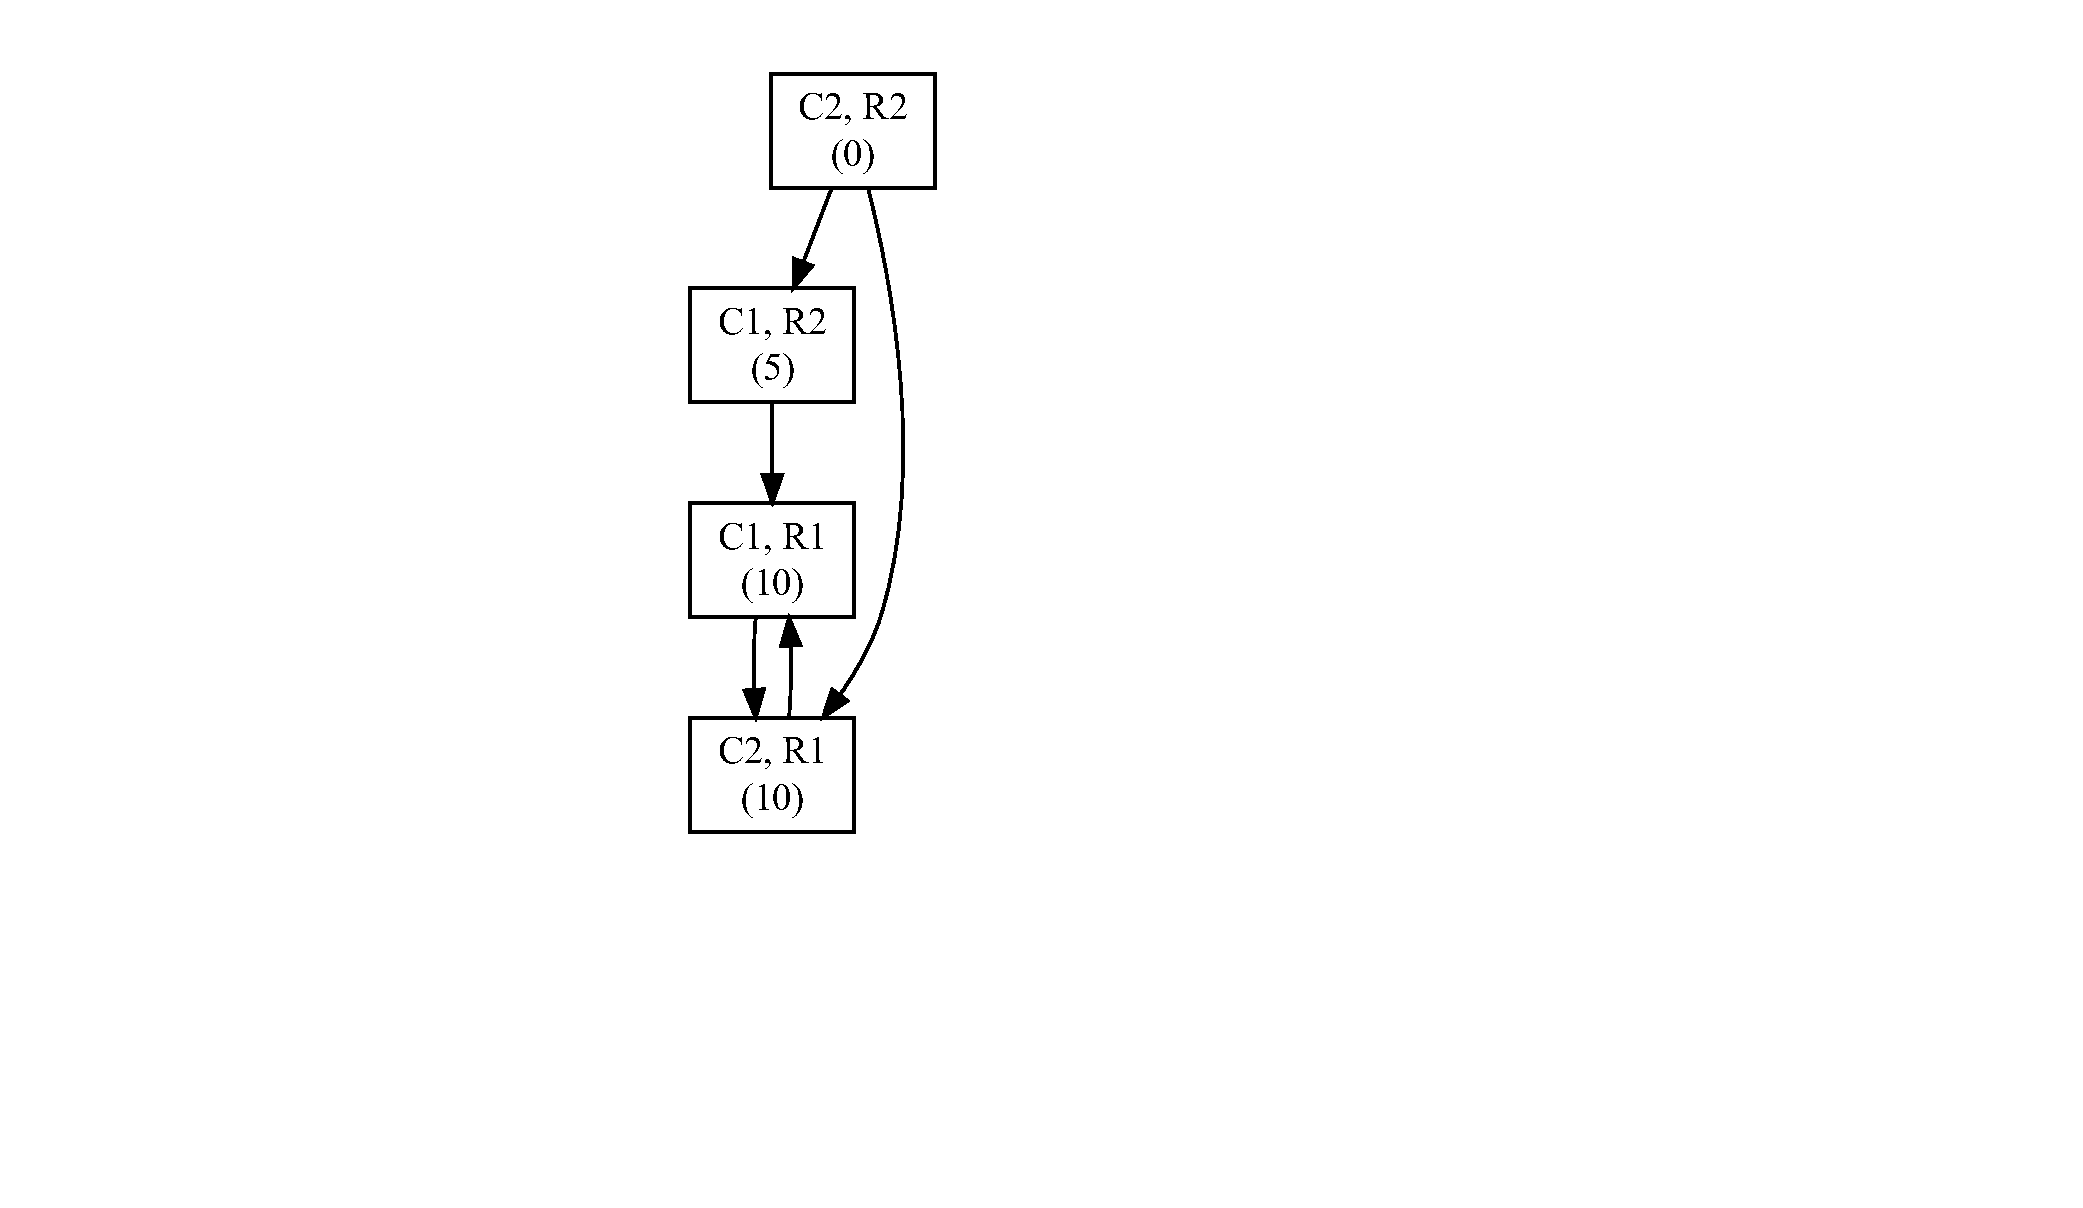
\includegraphics{Christophe_Hunt_hw9_files/figure-latex/unnamed-chunk-1-1.pdf}

We do have a pure strategy Nash equilibrium of 10 as our arrows all
point to one value, when Rose plays strategy 1 and Colin plays either
strategy 1 or 2. For graphing simplicity I set the strategy to Rose 1
and Colin 1.

\newpage

\section{Page 385: problem 1 c}\label{page-385-problem-1-c}

Using the definition provided for the movement diagram, determine
whether the following zero-sum games have a pure strategy Nash
equilibrium. If the game does have a pure strategy Nash equilibrium,
state the Nash equilibrium. Assume the row player is maximizing his
playoffs which are showing in the matrices below.

\begin{table}[!h]
\centering
\begin{tabular}{lllc}
 &  & \multicolumn{2}{l}{Pitcher} \\ \cline{3-4}
 &  & Fastball & \multicolumn{1}{l}{Knuckleball} \\ \hline
Batter & GFast & \multicolumn{1}{c}{.400} & .100 \\
 & Gknuckle & \multicolumn{1}{c}{.300} & .250 \\ \hline
\end{tabular}
\end{table}

\begin{Shaded}
\begin{Highlighting}[]
\KeywordTok{grViz}\NormalTok{(}\StringTok{"digraph boxes \{}

\StringTok{  graph [layout = neato, overlap = true, outputorder = edgefirst]}

\StringTok{  node [shape = box]}

\StringTok{  A [pos = '-1, 1!', label = 'Fastball, GFast }\CharTok{\textbackslash{}n}\StringTok{ (.400)']; }
\StringTok{  B [pos = ' 1, 1!', label = 'Knuckle, GFast  }\CharTok{\textbackslash{}n}\StringTok{ (.100)']; }
\StringTok{  C [pos = ' -1, -1!', label = 'Fast, GKnuckle }\CharTok{\textbackslash{}n}\StringTok{ (.300)']; }
\StringTok{  D [pos = ' 1, -1!', label = 'Knuckle, GKnuckle }\CharTok{\textbackslash{}n}\StringTok{ (.250)']; }

\StringTok{  # several 'edge' statements}
\StringTok{  C->D A->B C->A B->D}
\StringTok{\}}
\StringTok{"}\NormalTok{)}
\end{Highlighting}
\end{Shaded}

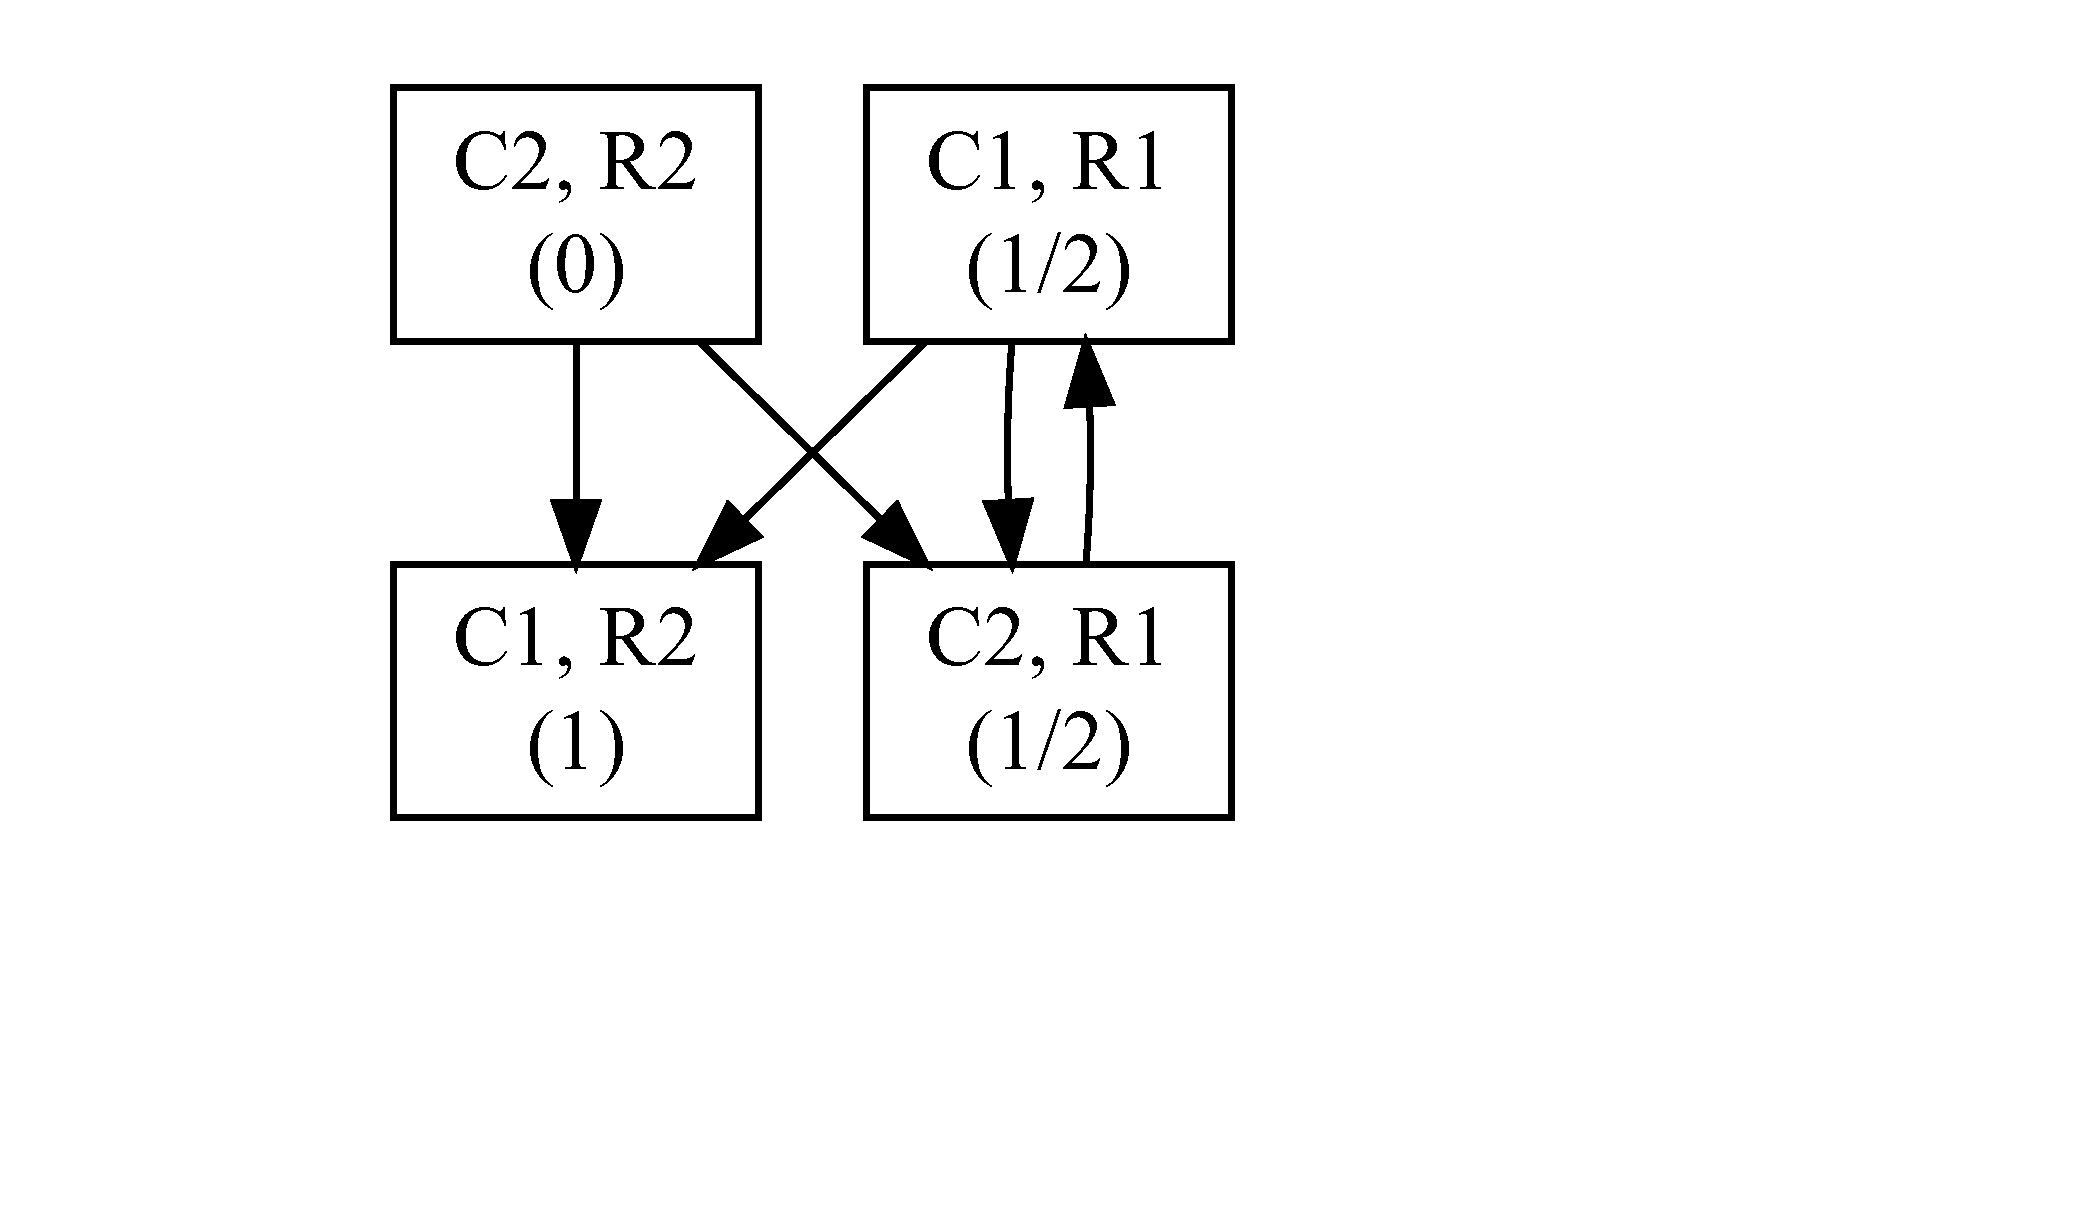
\includegraphics{Christophe_Hunt_hw9_files/figure-latex/unnamed-chunk-2-1.pdf}

The EV = .250 when the pitcher pitches a knuckle and the batter guesses
a knuckle ball.

\newpage

\section{Page 404: problem 2 a}\label{page-404-problem-2-a}

For problems a-g build a linear programming model for each player's
decisions and solve it both geometrically and algebraically. Assume the
row player is maximizing his playoffs which are showing in the matrices
below.

\begin{table}[!h]
\centering
\begin{tabular}{lllc}
 &  & \multicolumn{2}{l}{Colin} \\ \cline{3-4}
 &  & C1 & \multicolumn{1}{l}{C2} \\ \hline
Rose & R1 & \multicolumn{1}{c}{10} & 10 \\
 & R2 & \multicolumn{1}{c}{5} & 0 \\ \hline
\end{tabular}
\end{table}

Geometrically:

R1 has probability \(p = x\), therefore the probability of R2 is
\(p=1-x\).

\(V_{C1}\) \(\leq\) 10x + 5(1-x) = 5x + 5\\
\(V_{C2}\) \(\leq\) 10x + 0(1-x)= 10x\\
\(x \leq 1\)\\
\(x \geq 0\)

\begin{Shaded}
\begin{Highlighting}[]
\KeywordTok{library}\NormalTok{(knitr)}
\NormalTok{x <-}\StringTok{ }\KeywordTok{c}\NormalTok{(}\DecValTok{0}\NormalTok{, }\DecValTok{1}\NormalTok{, }\DecValTok{0}\NormalTok{, }\DecValTok{1}\NormalTok{)}
\NormalTok{A <-}\StringTok{ }\KeywordTok{c}\NormalTok{(}\DecValTok{5}\NormalTok{, }\DecValTok{10}\NormalTok{, }\DecValTok{0}\NormalTok{, }\DecValTok{10}\NormalTok{)}
\KeywordTok{kable}\NormalTok{(}\KeywordTok{as.data.frame}\NormalTok{(}\KeywordTok{cbind}\NormalTok{(x,A)))}
\end{Highlighting}
\end{Shaded}

\begin{longtable}[]{@{}rr@{}}
\toprule
x & A\tabularnewline
\midrule
\endhead
0 & 5\tabularnewline
1 & 10\tabularnewline
0 & 0\tabularnewline
1 & 10\tabularnewline
\bottomrule
\end{longtable}

\begin{Shaded}
\begin{Highlighting}[]
\KeywordTok{library}\NormalTok{(ggplot2)}
\NormalTok{plotc <-}\StringTok{ }\KeywordTok{ggplot}\NormalTok{(}\KeywordTok{data.frame}\NormalTok{(}\DataTypeTok{x=}\KeywordTok{c}\NormalTok{(}\DecValTok{0}\NormalTok{,}\DecValTok{1}\NormalTok{)), }\KeywordTok{aes}\NormalTok{(x)) +}
\StringTok{          }\KeywordTok{stat_function}\NormalTok{(}\DataTypeTok{fun=}\NormalTok{function(x)}\DecValTok{5}\NormalTok{*x}\DecValTok{+5}\NormalTok{, }\DataTypeTok{geom=}\StringTok{"line"}\NormalTok{, }\KeywordTok{aes}\NormalTok{(}\DataTypeTok{colour =} \StringTok{"C1"}\NormalTok{)) +}
\StringTok{          }\KeywordTok{stat_function}\NormalTok{(}\DataTypeTok{fun=}\NormalTok{function(x)}\DecValTok{10}\NormalTok{*x, }\DataTypeTok{geom=}\StringTok{"line"}\NormalTok{, }\KeywordTok{aes}\NormalTok{(}\DataTypeTok{colour =} \StringTok{"C2"}\NormalTok{)) +}
\StringTok{            }\KeywordTok{geom_vline}\NormalTok{(}\DataTypeTok{xintercept =} \DecValTok{1}\NormalTok{) +}\StringTok{ }
\StringTok{          }\KeywordTok{geom_vline}\NormalTok{(}\DataTypeTok{xintercept =} \DecValTok{0}\NormalTok{)}
\NormalTok{plotc}
\end{Highlighting}
\end{Shaded}

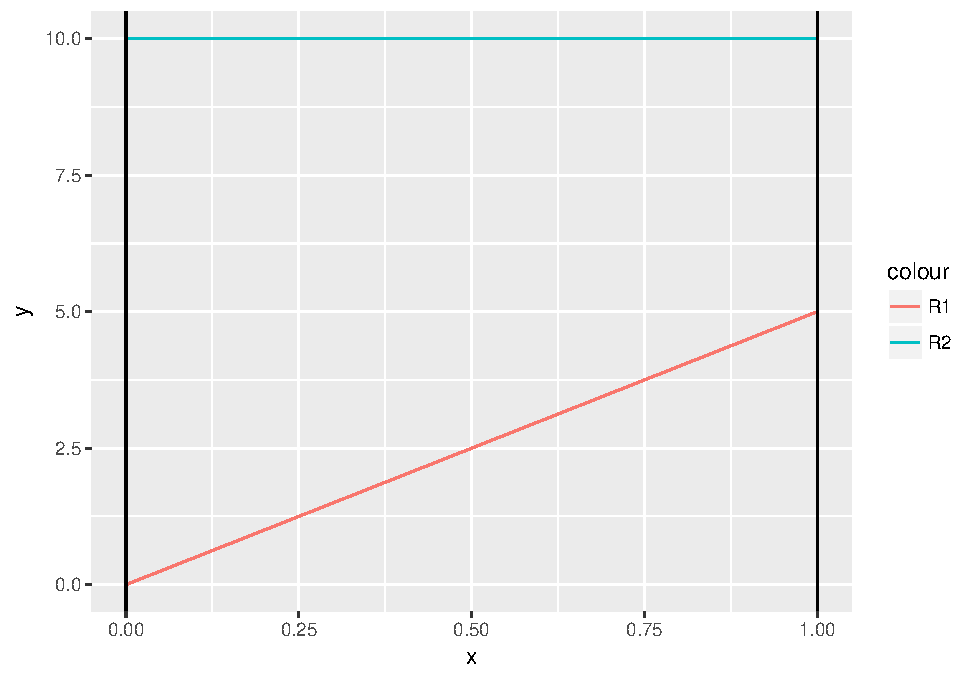
\includegraphics{Christophe_Hunt_hw9_files/figure-latex/unnamed-chunk-4-1.pdf}

Both are maxed at x = 1, \(V_{C1}\) = 10, \(V_{C2}\) = 10.

\newpage

R1 has probability \(p = x\), therefore the probability of R2 is
\(p=1-x\).

\(V_{R1}\) \(\leq\) 10x + 10(1-x) = 10 \(V_{R2}\) \(\leq\) 5x + 0(1-x)=
5x \(x \leq 1\) \(x \geq 0\)

\begin{Shaded}
\begin{Highlighting}[]
\KeywordTok{library}\NormalTok{(knitr)}
\NormalTok{x <-}\StringTok{ }\KeywordTok{c}\NormalTok{(}\DecValTok{0}\NormalTok{, }\DecValTok{1}\NormalTok{, }\DecValTok{0}\NormalTok{, }\DecValTok{1}\NormalTok{)}
\NormalTok{A <-}\StringTok{ }\KeywordTok{c}\NormalTok{(}\DecValTok{10}\NormalTok{, }\DecValTok{10}\NormalTok{, }\DecValTok{0}\NormalTok{, }\DecValTok{5}\NormalTok{)}
\KeywordTok{kable}\NormalTok{(}\KeywordTok{as.data.frame}\NormalTok{(}\KeywordTok{cbind}\NormalTok{(x,A)))}
\end{Highlighting}
\end{Shaded}

\begin{longtable}[]{@{}rr@{}}
\toprule
x & A\tabularnewline
\midrule
\endhead
0 & 10\tabularnewline
1 & 10\tabularnewline
0 & 0\tabularnewline
1 & 5\tabularnewline
\bottomrule
\end{longtable}

\begin{Shaded}
\begin{Highlighting}[]
\NormalTok{plotr <-}\StringTok{ }\KeywordTok{ggplot}\NormalTok{(}\KeywordTok{data.frame}\NormalTok{(}\DataTypeTok{x=}\KeywordTok{c}\NormalTok{(}\DecValTok{0}\NormalTok{,}\DecValTok{1}\NormalTok{)), }\KeywordTok{aes}\NormalTok{(x)) +}
\StringTok{          }\KeywordTok{stat_function}\NormalTok{(}\DataTypeTok{fun=}\NormalTok{function(x)}\DecValTok{5}\NormalTok{*x, }\DataTypeTok{geom=}\StringTok{"line"}\NormalTok{, }\KeywordTok{aes}\NormalTok{(}\DataTypeTok{colour =} \StringTok{"R1"}\NormalTok{)) +}
\StringTok{          }\KeywordTok{stat_function}\NormalTok{(}\DataTypeTok{fun=}\NormalTok{function(x)}\DecValTok{10}\NormalTok{, }\DataTypeTok{geom=}\StringTok{"line"}\NormalTok{, }\KeywordTok{aes}\NormalTok{(}\DataTypeTok{colour =} \StringTok{"R2"}\NormalTok{)) +}\StringTok{ }
\StringTok{            }\KeywordTok{geom_vline}\NormalTok{(}\DataTypeTok{xintercept =} \DecValTok{1}\NormalTok{) +}\StringTok{ }
\StringTok{          }\KeywordTok{geom_vline}\NormalTok{(}\DataTypeTok{xintercept =} \DecValTok{0}\NormalTok{)}
\NormalTok{plotr}
\end{Highlighting}
\end{Shaded}

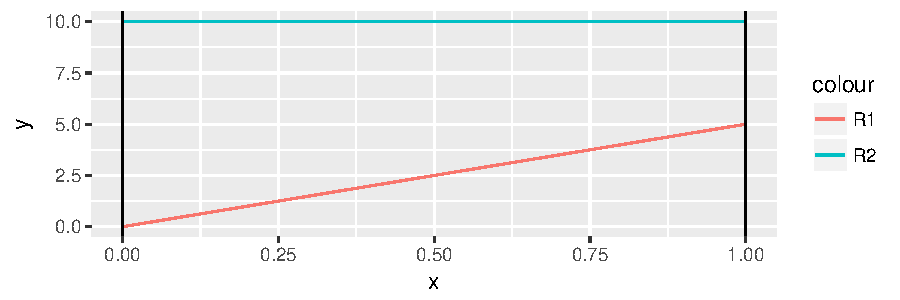
\includegraphics{Christophe_Hunt_hw9_files/figure-latex/unnamed-chunk-6-1.pdf}
\newpage

Now we plot both strategies for Rose and Colin.

\begin{Shaded}
\begin{Highlighting}[]
\KeywordTok{library}\NormalTok{(ggplot2)}
\NormalTok{plotrc <-}\StringTok{ }\KeywordTok{ggplot}\NormalTok{(}\KeywordTok{data.frame}\NormalTok{(}\DataTypeTok{x=}\KeywordTok{c}\NormalTok{(}\DecValTok{0}\NormalTok{,}\DecValTok{1}\NormalTok{)), }\KeywordTok{aes}\NormalTok{(x)) +}
\StringTok{          }\KeywordTok{stat_function}\NormalTok{(}\DataTypeTok{fun=}\NormalTok{function(x)}\DecValTok{5}\NormalTok{*x, }\DataTypeTok{geom=}\StringTok{"line"}\NormalTok{, }\KeywordTok{aes}\NormalTok{(}\DataTypeTok{colour =} \StringTok{"R1"}\NormalTok{)) +}
\StringTok{          }\KeywordTok{stat_function}\NormalTok{(}\DataTypeTok{fun=}\NormalTok{function(x)}\DecValTok{10}\NormalTok{, }\DataTypeTok{geom=}\StringTok{"line"}\NormalTok{, }\KeywordTok{aes}\NormalTok{(}\DataTypeTok{colour =} \StringTok{"R2"}\NormalTok{)) +}
\StringTok{          }\KeywordTok{stat_function}\NormalTok{(}\DataTypeTok{fun=}\NormalTok{function(x)}\DecValTok{5}\NormalTok{*x +}\StringTok{ }\DecValTok{5}\NormalTok{, }\DataTypeTok{geom=}\StringTok{"line"}\NormalTok{, }\KeywordTok{aes}\NormalTok{(}\DataTypeTok{colour =} \StringTok{"C1"}\NormalTok{)) +}
\StringTok{          }\KeywordTok{stat_function}\NormalTok{(}\DataTypeTok{fun=}\NormalTok{function(x)}\DecValTok{10}\NormalTok{*x, }\DataTypeTok{geom=}\StringTok{"line"}\NormalTok{, }\KeywordTok{aes}\NormalTok{(}\DataTypeTok{colour =} \StringTok{"C2"}\NormalTok{)) +}
\StringTok{          }\KeywordTok{geom_vline}\NormalTok{(}\DataTypeTok{xintercept =} \DecValTok{1}\NormalTok{) +}\StringTok{ }
\StringTok{          }\KeywordTok{geom_vline}\NormalTok{(}\DataTypeTok{xintercept =} \DecValTok{0}\NormalTok{)}
\NormalTok{plotrc}
\end{Highlighting}
\end{Shaded}

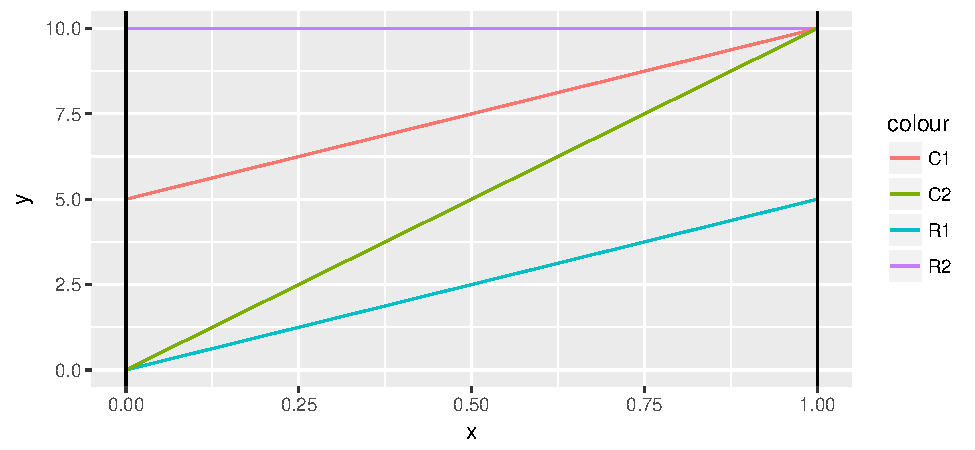
\includegraphics{Christophe_Hunt_hw9_files/figure-latex/unnamed-chunk-7-1.pdf}

\(V_{R1}\) is a constant at 10, whereas, \(V_{R2}\) is maxed at x = 1;
\(V_{R2}\) = 5.

We can therefore determine that Rose will play strategy R1 and Colin can
play either strategy C1 or C2.

\section{Page 420: problem 1}\label{page-420-problem-1}

In the following problems, use the maximim and minimax method and
movement diagram to determine if any pure strategy solution exist.
Assume the row player is maximizing his payoffs which are shown in the
matrices below.

\begin{table}[h]
    \begin{tabular}{lllcc}
    ~    & ~  & Colin & ~  & Row Minimum  \\
    ~    & ~  & C1    & C2 & ~            \\
    Rose & R1 & 10    & 10 & \textbf{10}   \\
    ~    & R2 & 5     & 0  & \textbf{0}   \\ \hline
    \end{tabular}
\end{table}

\begin{table}[h]
    \begin{tabular}{lllc}
    ~    & ~  & Colin & ~   \\
    ~    & ~  & C1    & C2  \\
    Rose & R1 & 10    & 10  \\
    ~    & R2 & 5     & 0     \\ 
    Column Maximum  & & \textbf{10} & \textbf{0}
    \\ \hline
    \end{tabular}
\end{table}

As we can see from the row minimum that Colin can play either C1 or C2;
and the column maximum indicates that Rose plays R1 which would be a
pure strategy.


\end{document}
